\documentclass{jsarticle}
\usepackage{amsmath, smssymb, amsfonts}
\usepackage{newtxtext, newtxmath}
\usepackage{latexsym}
\usepackage{mathrsfs}
\usepackage{mathtools}
\usepackage[dvipdfmx]{graphicx, xcolor}
\usepackage{float}
\usepackage{wrapfig}	% must be after float package.
\usepackage{subcaption}
\usepackage{booktabs}
\usepackage{url}
\usepackage{listings, jvlisting, color}

\definecolor{OliveGreen}{rgb}{0.0,0.6,0.0}
\definecolor{Orenge}{rgb}{0.89,0.55,0}
\definecolor{SkyBlue}{rgb}{0.28, 0.28, 0.95}
\lstset{
  language={C++}, % 言語の指定
  basicstyle={\ttfamily},
  identifierstyle={\small},
  commentstyle={\smallitshape},
  keywordstyle={\small\bfseries},
  ndkeywordstyle={\small},
  stringstyle={\small\ttfamily},
  frame={tb},
  breaklines=true,
  columns=[l]{fullflexible},
  numbers=left,
  xrightmargin=0zw,
  xleftmargin=3zw,
  numberstyle={\scriptsize},
  stepnumber=1,
  numbersep=1zw,
  lineskip=-0.5ex,
  keywordstyle={\color{SkyBlue}},     %キーワード(int, ifなど)の書体指定
  commentstyle={\color{OliveGreen}},  %注釈の書体
  stringstyle=\color{Orenge}          %文字列
}


\begin{document}

\title{ゼミ レポート 01}
\author{山田朔也}
\maketitle

\section{本レポートについて}
本レポートでは、熱伝導方程式を数値的に解く問題の結果を示すものである。
また問題はいくつかに分かれているが、基本事項は同じのため、それらについては問題の結果の前にまとめて記述しておく。

\section{各種基本事項の説明}
\subsection{問題について}
本問題は以下の図\ref{fig01}のような一次元の棒の両端を0℃としたときの熱伝導方程式を、数値的に解くことを目的としている。
つまり、時間と空間を離散化して、各代表点の温度変化を計算して行けば良い。
\begin{figure}[H]
	\centering
	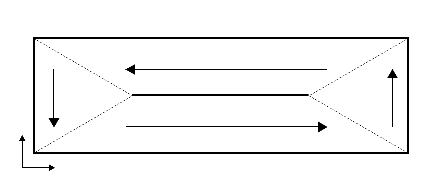
\includegraphics[width=8cm]{pic01.eps}
	\caption{本問題における初期条件}
	\label{fig01}
\end{figure}%

与えられる初期条件は、棒の長さが1で、棒の両端の温度が0℃。
それ以外の点は図\ref{fig01}のように中央に近づくにつれて高くなっていき、中央は1℃となる。
そして、棒の両端は温度0℃の氷と接触しており、温度は0℃を維持する。
以上が初期条件となっている。

また、長さ方向の座標軸を$x$軸、時刻を$t$、温度$T$を$x$と$t$からなる関数とする。
このとき熱伝導方程式は
\begin{equation}
	\frac{\partial T(x,t)}{\partial t} = \frac{\partial ^2 T(x,t)}{\partial x^2}	\label{01}
\end{equation}
となり、境界条件は
\begin{equation}
	T(0,t) = T(1,t) = 0	\label{02}
\end{equation}
と表せる。

\subsection{計算モデルについて}
計算モデルを用意するために、式\ref{01}を離散化する必要があるため、それを行っていく。
まずは関数$T$を各代表点$i$と時間$t$からなる関数とみなす。
ここから、まずは中心差分近似を用いて、熱伝導方程式の空間微分を離散化する。
この条件で関数$T$をテイラー展開する。すると
\begin{equation}
	T(i+1,t) = T(i,t) + dxT^{\prime}(i,t) + \frac{dx^2}{2}T^{\prime\prime}(i,t) + \frac{dx^3}{6}T^{\prime\prime\prime}(i,t) + O(dx^4) + \ldots
\end{equation}
\begin{equation}
	T(i-1,t) = T(i,t) - dxT^{\prime}(i,t) + \frac{dx^2}{2}T^{\prime\prime}(i,t) - \frac{dx^3}{6}T^{\prime\prime\prime}(i,t) + O(dx^4) + \ldots
\end{equation}
の2式が得られる。この2式の左辺と右辺をそれぞれ足し合わせると、
\begin{equation}
	T(i+1,t) + T(i-1,t) = 2T(i,t) + dx^{2}T^{\prime\prime}(i,t) + O(dx^4)
\end{equation}
\begin{equation}
	\rightarrow T^{\prime\prime}(i,t) = \frac{{\partial}^{2} T}{\partial x^2} \sim \frac{T(i-1,t) - 2T(i,t) +T(i+1,t)}{dx^2} \label{03}
\end{equation}
という式が得られる。式\ref{03}にあるように、この式は熱伝導方程式の右辺に近似できる式となっている。
これにより、空間が離散化されたときの近似式が得られた。

次はオイラー法を用いて、式\ref{01}の時間を離散化していく。
オイラー法は、仮に求めたい式を$y$として、$\frac{dy}{dt} = f(t,y(x))$の形で既知の関数$f(t,y(x))$で表せるとき。
\begin{equation}
	y(t_0+\Delta t) = y(t_0) + \Delta ty^{\prime}(t) + \ldots	\label{04}
\end{equation}
という形で近似する手法となっている。
これは以下の図\ref{fig02}にあるように、$y(t_0+\Delta t)$の値を、
$t_0$における傾き$\frac{dy}{dt}$と$\Delta t$を掛け合せた値に、$y(t_0)$の値を足したもので近似している。
\begin{figure}[H]
	\centering
	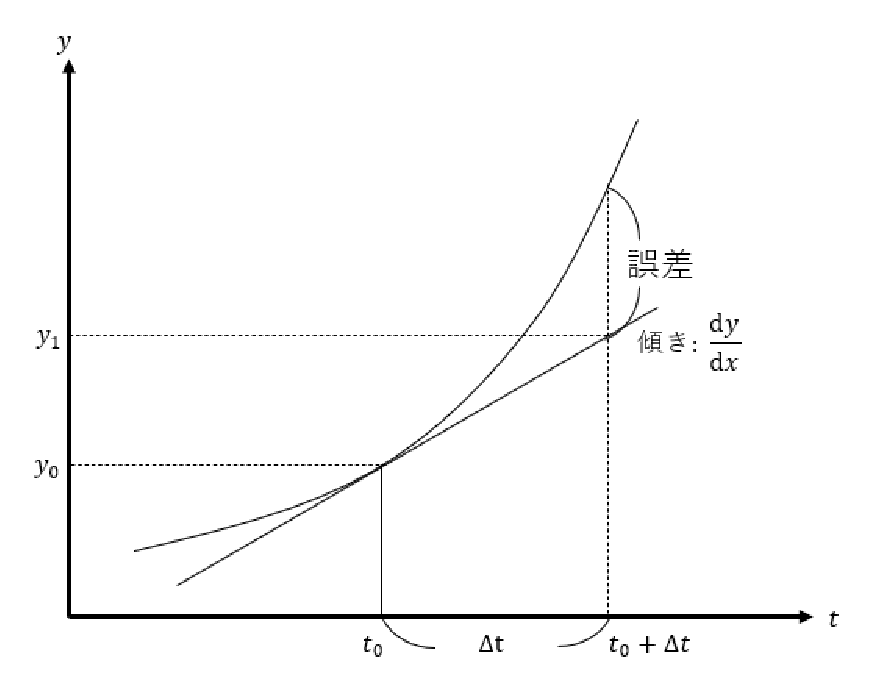
\includegraphics[width=10cm]{pic02.eps}
	\caption{オイラー法の視覚的説明}
	\label{fig02}
\end{figure}%
ただし、計算しているのはあくまで傾きであるため、図\ref{fig02}のように誤差が出る。そのため、$\Delta t$を十分に小さくする必要がある。
また、式\ref{04}では所謂傾きである一次微分までしか行っていないが、より精度を求めるなら二次以降も計算すると良い。

これを熱伝導方程式に適用すると
\begin{equation}
	T(i,t+\Delta t) = T(i,t) + \Delta \frac{T(i-1,t) - 2T(i,t) + T(i+1,t)}{dx^2}	\label{05}
\end{equation}
という式が得られる。

ここから、以下のようなアルゴリズムを用いることで数値的に解が得られる。
\begin{enumerate}
	\item 各種初期条件を設定する。
	\begin{itemize}
		\item 棒の分割数$n$、またこれによって代表点間の距離$dx=\frac{1}{n}$が決定する。
		\item 温度の初期条件を$T$に設定する。
		\item 時間の刻み幅$dt$の決定
	\end{itemize}
	\item 初期条件と式\ref{05}から各代表点の$dt$後の状態を計算する。
	\item 上の項目2を任意の回数行う。
\end{enumerate}

\subsection{使用したプログラムについて}
まず、前の章で策定したアルゴリズムを元に作成した、C言語のプログラムのソースコードを以下に記載する。
\begin{lstlisting}[H, caption=熱伝導方程式の数値的に解を得るプログラム, label=list01, language=C++]
#include <stdio.h>
#include <stdlib.h>
#include <stdbool.h>

int printout(int n, double* T, int t) {
	// 最初に呼ばれたときのみ実行
	static bool IsFirst = true;
	int i;
	if(IsFirst) {
		// 表最初の行を出力
		printf("time ");
		for(i = 0; i <= n; i++){
			printf("T%d ", i);
		}
		printf("\n");
		IsFirst = false;
	}

	// 中身を出力
	printf("%d*dt ", t);
	for(i = 0; i <= n; i++) {
		printf("%.4lf ", T[i]);
	}
	printf("\n");
}

int calcDT(double* T, double* DT, double dx, double dt, int n) {
	int i = 0;
	DT[0] = 0; DT[n] = 0;
	for (i = 1; i < n; i++) {
		DT[i] = dt*(T[i-1] - 2*T[i] + T[i+1])/(dx*dx);
	}
}

int calcT(double* T, double* DT, int n) {
	int i = 0;
	for (i = 1; i < n; i++) {
		T[i] = T[i] + DT[i];
	}
}

int main() {
	// 各種初期値の取得
	int n = 0;
	scanf("%d", &n);

	double dt = 0.0;
	scanf("%lf", &dt);

	double dx;
	dx = (double)1.0 / (double)n;

	double T[n+1];
	double DT[n+1];

	// 初期条件設定
	int i = 0;
	for (i = 0; i <= n/2; i++) {
		T[i] = 2*dx*i;
		T[n-i] = T[i];
	}
	printout(n, T, 0);

	// 計算のメインループ
	int t = 0;
	for (t = 1; t <= 10; t++) {
		calcDT(T, DT, dx, dt, n);
		calcT(T, DT, n);
		printout(n, T, t);
	}

	return 0;
}
\end{lstlisting}
このプログラムを実行した後、まずは分割数nを標準入力で入力。続いてdtも入力する。
するとそれを元に、初期条件及び、熱伝導方程式の数値的に解を得ることができる。

結果の出力方法は、標準出力へとなっている。出力形式は以下の表\ref{結果01}のようになっている。
計算を行うにあたって、配列$T$と$DT$を用意し、それぞれ別に計算を行っている。
これは、配列$T$は$T(i,t+\Delta t)$の値を保持し、$DT$は$\Delta \frac{T(i-1,t) - 2T(i,t) + T(i+1,t)}{dx^2}$を保持することで、上書きなどを避けるためである。
各関数の説明は以下のようになる。
\begin{itemize}
	\item 関数printout。配列$T$とその他の変数から、必要な情報を出力する。
	\item 関数calcDT。配列$DT$に入る数値を、前のループで計算してあった$T$から計算する。
	\item 関数calcT。前のループでの計算結果の残っている配列$T$と、新たに計算した$DT$から、今ループでの$T$を計算する。
\end{itemize}


\section{問題への解答}
\subsection{問題1}
問題の内容は、熱伝導方程式の解を数値的に得るプログラムを作成し、それが与えられたテキストの表1と一致しているかを確認するものである。

以下にプログラムを実行して計算した結果を表\ref{tab01}として記載する。
\begin{table}[H]
	\caption[出力結果]{作成したプログラムを$n=10$, $dt=0.001$で実行した出力結果}
	\label{tab01}
	\begin{center}
		\setlength{\tabcolsep}{3pt}
		\footnotesize
		\begin{tabular}{rccccccccccc}
			time & T0 & T1 & T2 & T3 & T4 & T5 & T6 & T7 & T8 & T9 & T10	\\
			0*dt & 0.0000 & 0.2000 & 0.4000 & 0.6000 & 0.8000 & 1.0000 & 0.8000 & 0.6000 & 0.4000 & 0.2000 & 0.0000	\\
			1*dt & 0.0000 & 0.2000 & 0.4000 & 0.6000 & 0.8000 & 0.9600 & 0.8000 & 0.6000 & 0.4000 & 0.2000 & 0.0000	\\
			2*dt & 0.0000 & 0.2000 & 0.4000 & 0.6000 & 0.7960 & 0.9280 & 0.7960 & 0.6000 & 0.4000 & 0.2000 & 0.0000	\\
			3*dt & 0.0000 & 0.2000 & 0.4000 & 0.5996 & 0.7896 & 0.9016 & 0.7896 & 0.5996 & 0.4000 & 0.2000 & 0.0000	\\
			4*dt & 0.0000 & 0.2000 & 0.4000 & 0.5986 & 0.7818 & 0.8792 & 0.7818 & 0.5986 & 0.4000 & 0.2000 & 0.0000	\\
			5*dt & 0.0000 & 0.2000 & 0.3998 & 0.5971 & 0.7732 & 0.8597 & 0.7732 & 0.5971 & 0.3998 & 0.2000 & 0.0000	\\
			6*dt & 0.0000 & 0.2000 & 0.3996 & 0.5950 & 0.7643 & 0.8424 & 0.7643 & 0.5950 & 0.3996 & 0.2000 & 0.0000	\\
			7*dt & 0.0000 & 0.1999 & 0.3992 & 0.5924 & 0.7551 & 0.8268 & 0.7551 & 0.5924 & 0.3992 & 0.1999 & 0.0000	\\
			8*dt & 0.0000 & 0.1999 & 0.3986 & 0.5893 & 0.7460 & 0.8125 & 0.7460 & 0.5893 & 0.3986 & 0.1999 & 0.0000	\\
			9*dt & 0.0000 & 0.1998 & 0.3978 & 0.5859 & 0.7370 & 0.7992 & 0.7370 & 0.5859 & 0.3978 & 0.1998 & 0.0000	\\
			10*dt & 0.0000 & 0.1996 & 0.3968 & 0.5822 & 0.7281 & 0.7867 & 0.7281 & 0.5822 & 0.3968 & 0.1996 & 0.0000	\\
		\end{tabular}
	\end{center}
\end{table}
今回の与えられたテキストの表1と、本レポートの表1は一致しているため、これを満たしている。

\subsection{問題2}
問題の内容は、問題一の結果をgnuplotを用いてグラフとして描画することである。

実際に計算結果をgnuplotでグラフにすると以下の図\ref{fig03}ようになった。
\begin{figure}[H]
	\centering
	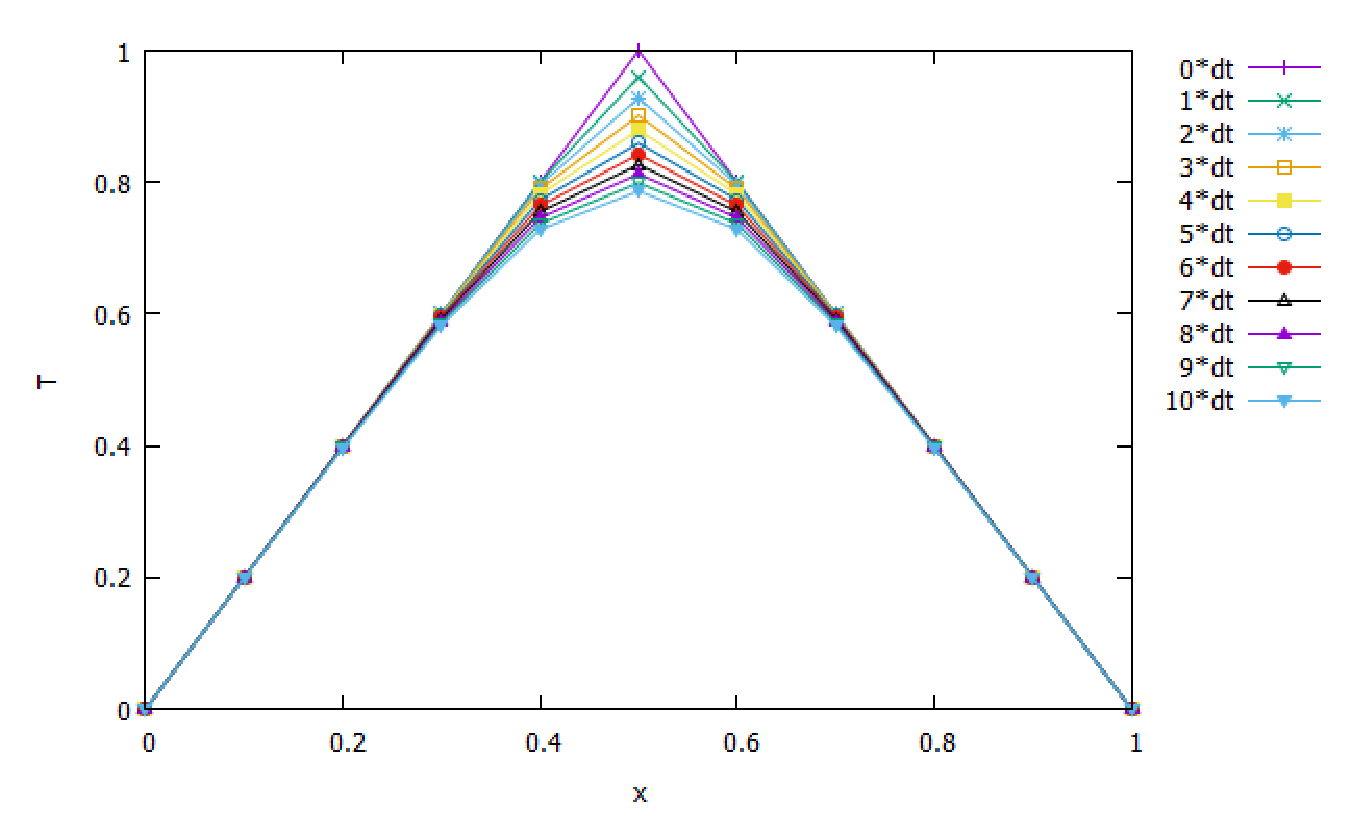
\includegraphics[width=14cm]{pic03.eps}
	\caption{表\ref{tab01}をグラフに出力したもの}
	\label{fig03}
\end{figure}

\subsection{問題3}
問題の内容は、$dt$の値を変化させて計算させたとき、計算が破綻する$dt$の値を調べることである。
この計算モデルの特徴から、$dt$の値を減少させればさせるほど精度が増していくため、今回は$dt$の値を増加させて検証していく。
まずは、$dt=0.001$から$dt$を0.001ずつ増加させて計算していった。このとき、$dt=0.006$のとき初めて明らかに計算が破綻していた。(図\ref{fig05})
\begin{figure}[H]
	\centering
	\begin{subfigure}{0.9\columnwidth}
		\centering
		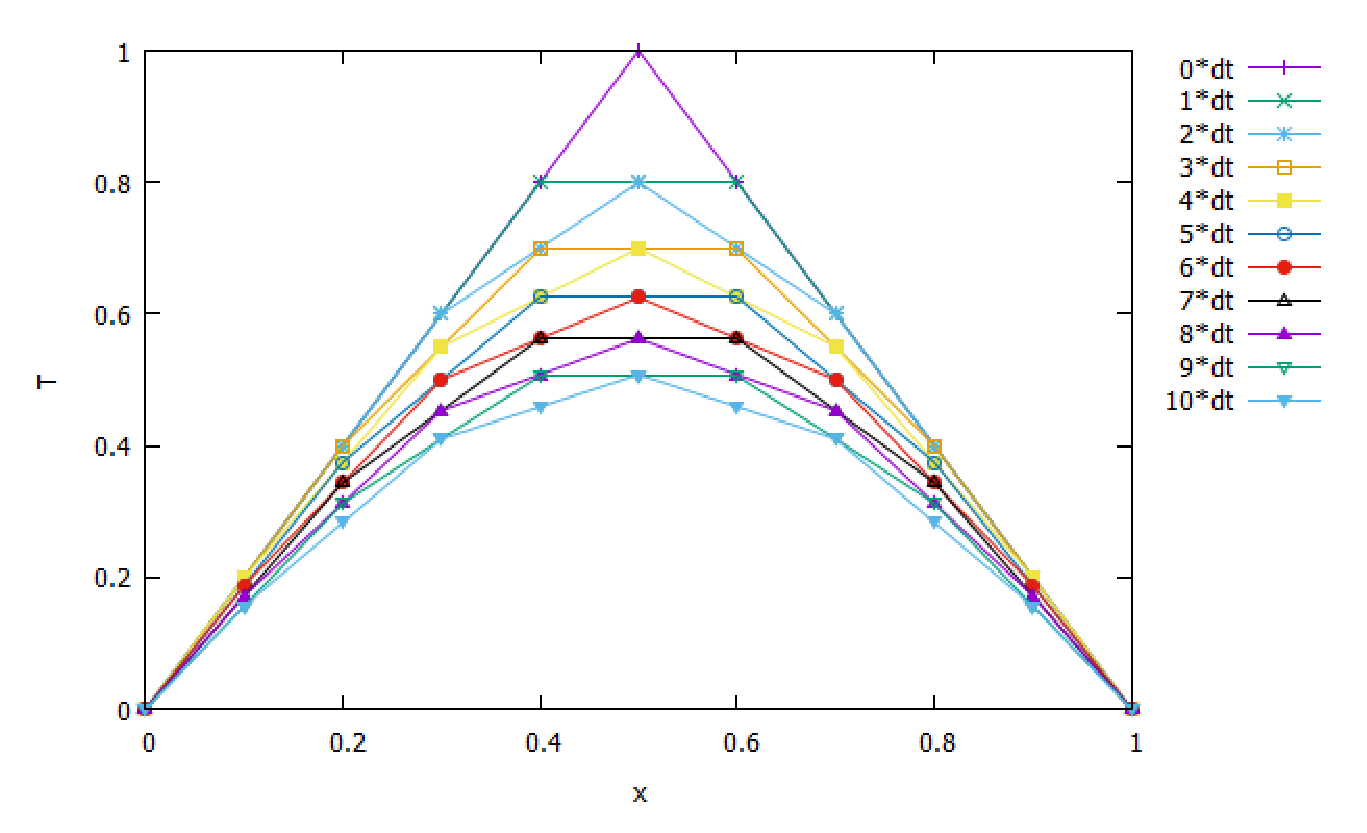
\includegraphics[width=\columnwidth]{pic04.eps}
		\caption{$dt=0.005$の時の実行結果}
		\label{fig04}
	\end{subfigure}
	\begin{subfigure}{0.9\columnwidth}
		\centering
		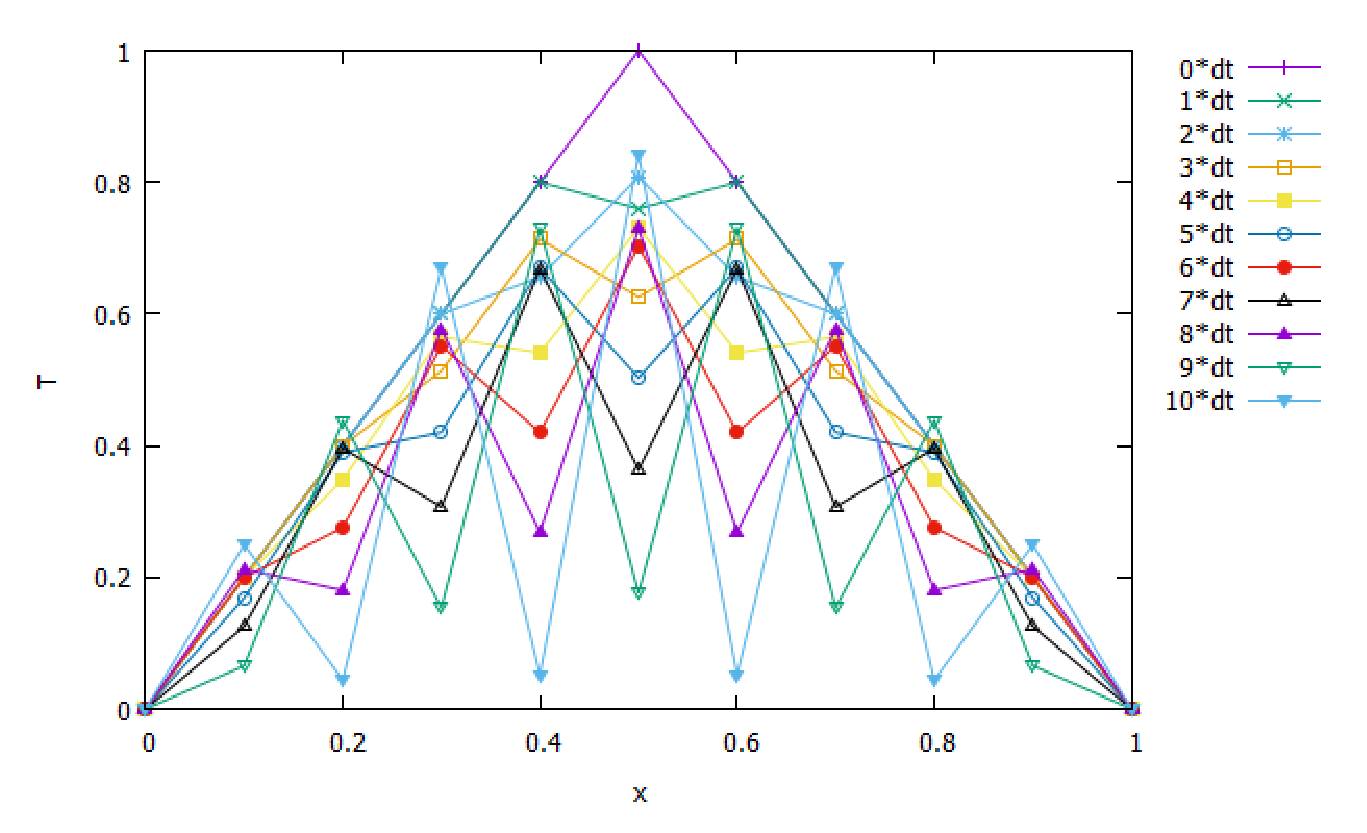
\includegraphics[width=\columnwidth]{pic05.eps}
		\caption{$dt=0.006$の時の実行結果}
		\label{fig05}
	\end{subfigure}
	\label{fignone01}
	\caption{0.001ずつ増加させたときの実行結果}
\end{figure}
更に、$dt=0.0051$の場合を計算すると、以下の図\ref{fig06}のようになった。
\begin{figure}[H]
	\centering
	
\includegraphics[width=14cm]{pic06.eps}
	\caption{$dt=0.0051$の時の実行結果}
	\label{fig06}
\end{figure}
左端の代表点を第0番目としたときの、第4番目の代表点を見ると顕著であるが。
$dt=0.005$の時の計算結果では、時間経過によって代表点の温度が同じであっても、それ以前より上昇することはなかった。
しかし、それを少しでも超えるた場合、ある代表点では時間経過によって、それ以前の温度より上昇するという計算結果となった。
このことから、計算が破綻する$dt$の値は$dt=0.005$より大きい値の時だとわかる。

\subsection{問題4}
問題の内容は、分割数$n$の値を変化させて計算させたとき、計算が破綻する$n$の値を調べることである。
まずは、$n=10$から$n$を1ずつ減少させて計算していった。このときは計算は破綻しなかった。
次に$n=10$から$n$を1ずつ増加させて計算していった。結果は、$n=24$のとき、計算の破綻が確認された。
以下の図\ref{fig08}がその時のグラフとなっている。
\begin{figure}[H]
	\centering
	\begin{subfigure}{0.9\columnwidth}
		\centering
		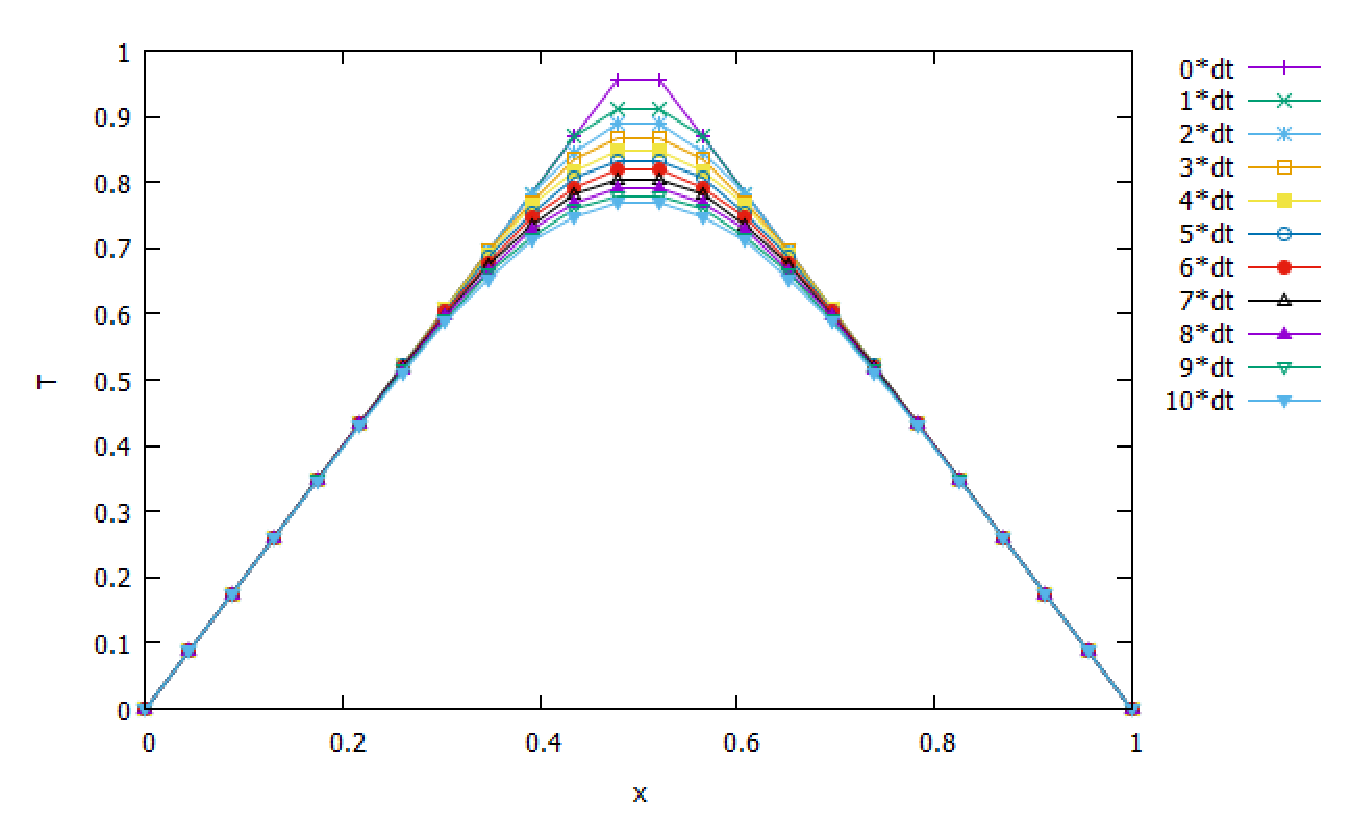
\includegraphics[width=\columnwidth]{pic07.eps}
		\caption{$n=23$の時の実行結果}
		\label{fig07}
	\end{subfigure}
	\begin{subfigure}{0.9\columnwidth}
		\centering
		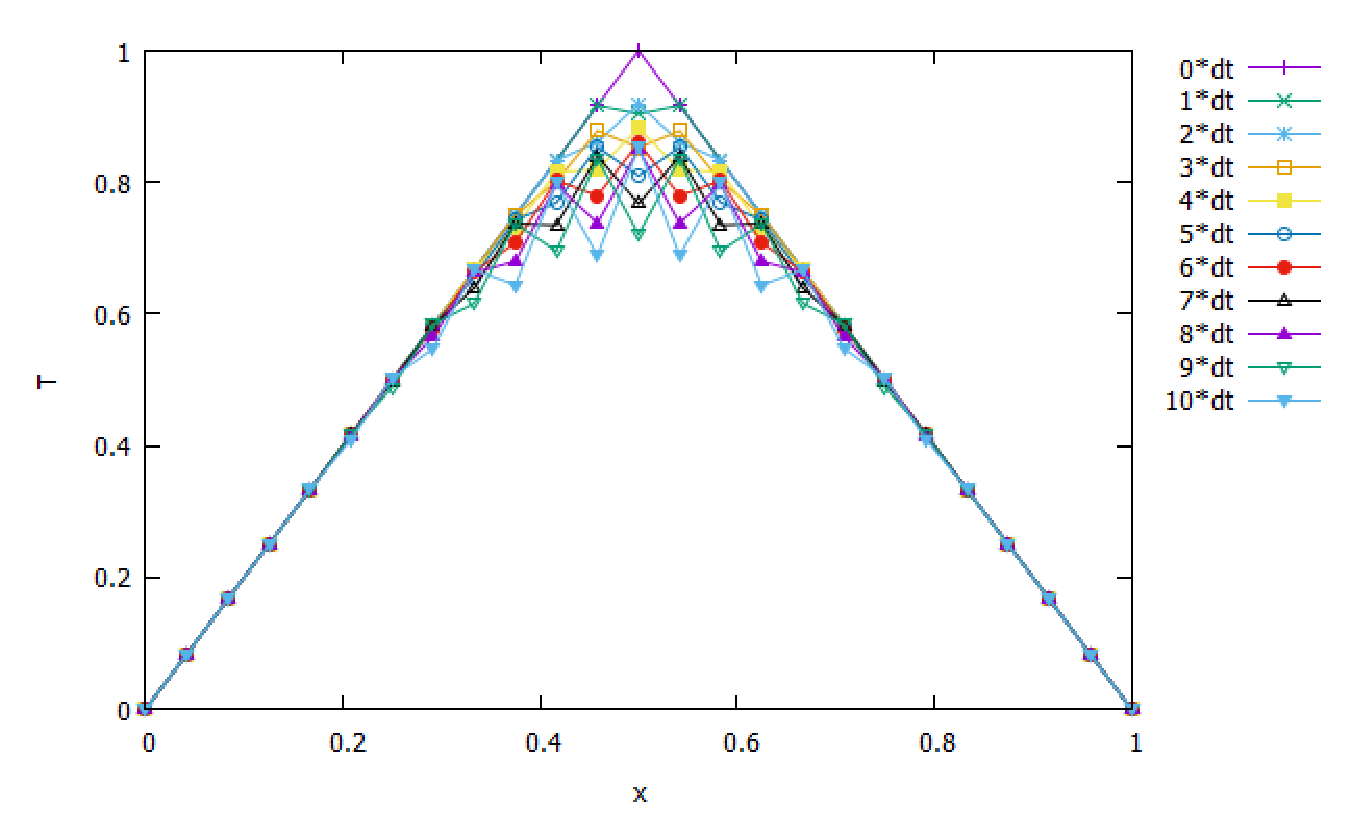
\includegraphics[width=\columnwidth]{pic08.eps}
		\caption{$n=24$の時の実行結果}
		\label{fig08}
	\end{subfigure}
	\label{fignone02}
	\caption{$n$を1ずつ増加させたときの実行結果}
\end{figure}
グラフの中央付近からもわかるように、時間が経過しているにもかかわらず温度が上昇するといった明らかな計算の破綻が見られている。


\subsection{問題5}
問題の内容は、$dt,n$を共に変化させて計算を行い、計算が破綻しない条件を探すことである。

まず、nの値を$6\backsim 48$の範囲で変化させ、その中で更に$dt$を$dt=0.0001$から0.0001ずつ増やしつつ、
計算が破綻する直前の$dt$の値を調べた。また、計算の破綻は、どこかの代表点が時間経過前の温度を超過した場合とする。
それらの値を、$n$の値を横軸に、$dt$の値を縦軸に取ると以下の図\ref{fig09}のようなグラフになった。
\begin{figure}[H]
	\centering
	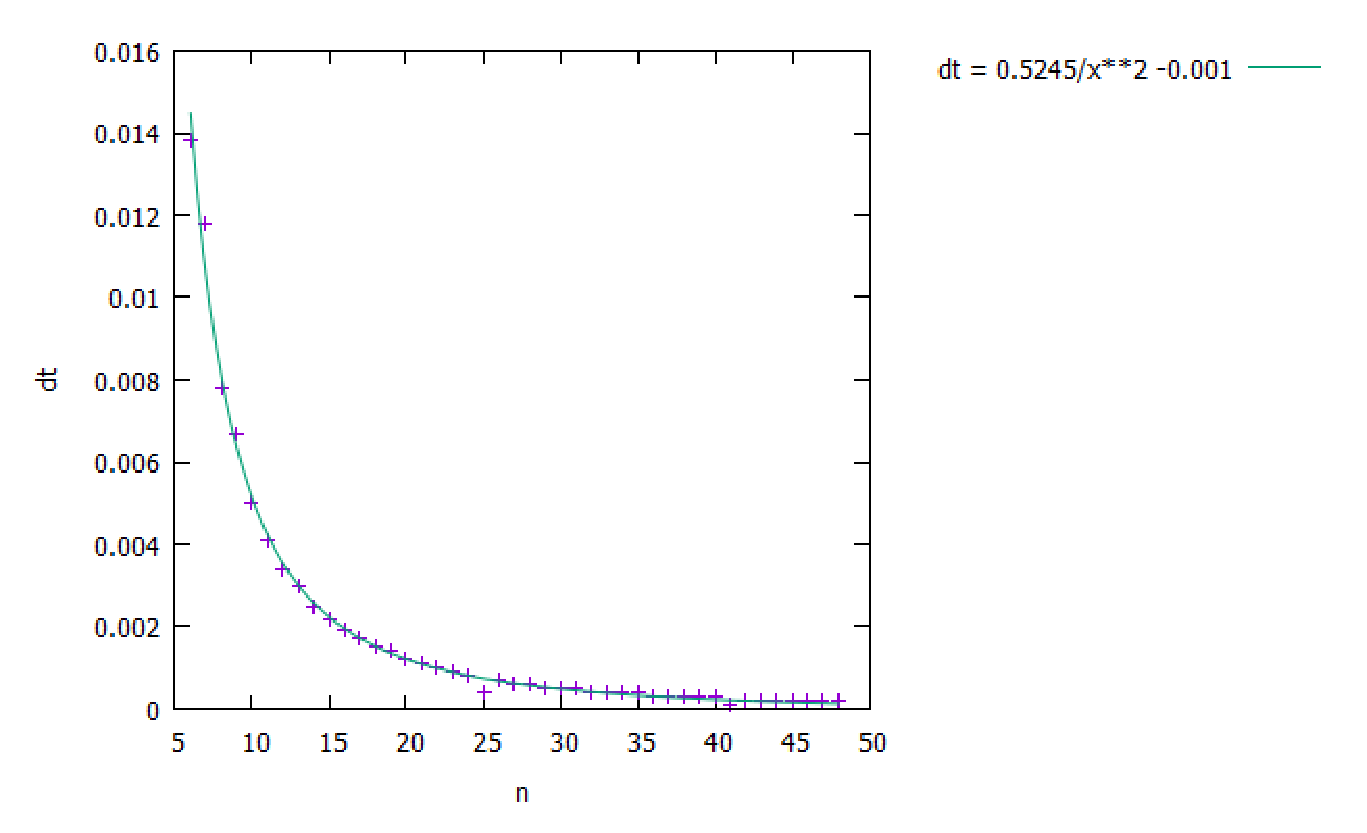
\includegraphics[width=14cm]{pic09.eps}
	\caption{各$n$の値に対して、ちょうど計算が破綻しない$dt$の値とその近似曲線}
	\label{fig09}
\end{figure}
この図にもあるように、ちょうど計算が破綻しない$dt$の値から近似曲線を取ると以下のような式になった。
\begin{equation}
	dt = \frac{0.5245}{x^2} - 0.001	\label{06}
\end{equation}
このことから、解が安定して求められる条件は、$dt$の値が式\ref{06}の右辺の値を超えなければ良いと分かる。

\section{参考文献}

\begin{itemize}
  \item 配布されたテキスト
\end{itemize}

\end{document}